\chapter{Radar System Overview}

In order to build a model capable of accurately capturing key features from target surfaces one must first understand the origin and structure of the received signal. In this chapter a few fundamental concepts in radar systems are introduced that explain how a target's range, velocity and reflectivity arise in a \gls{pcr} system. The mixing and \gls{iq} demodulation procedures are also discussed, which explain how radar measurements are performed.  

\section{Target Properties from Pulsed Radar Response}
% TODO: Utilize https://acconeer.sharepoint.com/:w:/g/CS/ES_xwcoTqVdGkShPJkNagMMBL1wVd_GaeJJsEDKC8lWIDQ?e=GxZNEw as a source for this.
Fundamentally, a radar operates by radiating \gls{rf} electromagnetic energy and listening if the transmitted energy generates any echoes \citep{skolnik_2009}. By analyzing properties of returning signals it is then possible to obtain information regarding the scattering targets. This may involve the distance and angle at which scatterers are located or at which velocity they are moving in. With a sufficiently high angular and range resolution it is even possible to discern shapes and sizes.  

Standard radars are active systems, meaning that they have a radiating antenna and hence do not depend on any ambient radiation emitted by the target \citep{richards_2014}. Radar systems can be realized in many ways, however in this report a \gls{pcr} system is used. This means that a sequence of short coherent wavelets are transmitted towards a target scene to determine its properties. One such transmitted wavelet pulse $x_T(t)$ has some carrier frequency, $f_c$, and envelope $A(t)$ as in
\begin{equation}\label{eq:trans}
	x_T(t)
	= A(t)\sin(2\pi f_c t).
\end{equation}

After various scattering processes, the returning signal is captured by either an array of antennas, or just a single antenna.

\subsection{Single-Antenna Considerations}

Commonly, in larger radar systems, many receiving antennas capture the returning radiation. This allows for distinguishing radar targets not only in range, but also in angle. In this work a single receiving antenna is used, meaning that the radar has no intrinsic method of determining at which angle a scatterer is located. Thus, only information in range can be captured by this sensor.

To understand what information can be obtained from such a one-dimensional signal, a single scattering object some distance away from the transmitter is here considered. If a radar pulse on the form of \eqref{eq:trans} is transmitted towards it, the returning signal will be a delayed pulse on the form \citep{richards_2014}
\begin{equation}\label{eq:returning}
	y(t) = CA(t-B)\sin(2\pi f_c (t-B))
\end{equation}
where $B$ is some delay related to the distance to the target and $C$ a constant corresponding to the loss of energy from transmission to reception of a pulse. For the purposes of this report the properties of this delay is of particular interest. In the next two sections it is shown how distance and velocity can be deduced from this parameter using absolute measurements of $B$ and relative changes in $B$ between pulse measurements. The $C$ variable carries information about the reflectivity of a scatterer, described lastly. 

\subsection{Radar Distance Measurements}

If a point scatterer was present a distance $d$ from the transmitting antenna, a wavelet will return $2d/c$ seconds after transmission, where $c$ denotes the speed of light. The 2 appears to accommodate for the pulse traveling forth and back between the sensor and the scatterer. Hence, the transmitted signal is delayed according to 
\begin{equation}
	\begin{split}
		y(t) 
		& = CA(t-2d/c)\sin(2\pi f_c(t - \frac{2d}{c})) \\
		& = CA(t-2d/c)\sin(2\pi f_ct - \frac{4\pi d}{c}f_c).
	\end{split}
\end{equation}

By measuring the delay $B$ in \eqref{eq:returning} either as a phase shift or a shift in envelope we can thus simply calculate the distance through
\begin{equation}
	d = \frac{Bc}{2}.
\end{equation}

Thus, by examining the time delay of the returning signal, we can deduce the distance to the scattering object. 

\subsection{Doppler Frequency in Pulsed Radar}\label{sec:doppler}
\label{doppler}

If the target scatterer is moving from or towards the transmitting antenna, a shift in frequency will occur in the received pulse $y(t)$. For velocity $v$, the transmitted frequency $f_c$ will be shifted to $f_r$ according to the well known Doppler formula \citep{ridenour_1947}
\begin{equation}
	f_r = \frac{c + v}{c - v}f_c
\end{equation}
where positive $v$ indicates that the scatterer is moving towards the transmitter. The frequency shift $f_d$, also known as the \emph{beat frequency} (\gls{bf}), is then
\begin{equation}\label{eq:dshift}
	f_d 
	= f_r - f_c 
	= \frac{2v}{c-v}f_c \approx \frac{2v}{c}f_c 
	= \frac{2v}{\lambda_c}
\end{equation}
where $\lambda_c$ is the carrier wavelength. This shift means that an approaching target has slightly increased returning frequency, and conversely that a receding target has a slightly decreased frequency. In this project a pulsed radar is used, meaning that measurements are done repeatedly using short wavelets instead of transmitting one continuous wave. What does this mean for the Doppler shift?

The use of short wavelets means that each individual transmitted pulse becomes compressed by the Doppler shift. This compression is miniscule, on the scale of fractions of picoseconds, and thus insignificant for any target with reasonably moderate velocity. For a \gls{pcr} system with sampling frequency, $F_s$, and sampling period, $T_s = 1/F_s$, the Doppler shift can instead of a shift in frequency be viewed as a phase shift from one pulse to the next. Between two distance measurements a target moves a distance $vT_s$. Hence, each pulse travels a distance $2vT_s$ less than the preceding one. This distance corresponds to $2vT_s/\lambda_c$ wavelengths, providing a phase change, $\Delta \phi$, per pulse of
\begin{equation}
	\Delta \phi = \frac{4\pi}{\lambda_c}vT_s.
\end{equation}

For a target moving at a constant pace, the \gls{bf} arising from the constant Doppler phase shift is thus $f_d = 2v/\lambda_c$, as was found in equation \eqref{eq:dshift}. Thus, by taking a discrete Fourier transform (\gls{dft}) of the sequence of $T_s$-spaced measurements for one specific distance, we can estimate the velocity from the peak frequency $f$ in the \gls{dft} as 
\begin{equation}\label{eq:dopp}
	v = \frac{\lambda_c f_d}{2}
	\approx \frac{\lambda_c f}{2}.
\end{equation}


\subsection{Power Dissapation}

The $C$ factor in \eqref{eq:returning} describes the ratio of the emitted power that is received after scattering. To get a feel for how a target's reflectivity relates to this factor we can make the following thought experiment. First, we assume that the transmitted power $P_t$ is radiated isotropically by a point source, meaning that the power density is distributed uniformly by the source over the surface of a sphere. When our radar ``balloon'' has radius $R$, the power density at the balloon surface becomes  \citep{amin_2017}
\begin{equation}
	P_d 
	= \frac{P_t}{4\pi R^2}
\end{equation}
where $4\pi R^2$ is the surface area of the balloon. If a scatterer is present at range $d$ with radar cross section (\gls{rcs}) $\sigma$ and gain $G_t$, the fraction of the radar power reflected by the scatterer is given by 
\begin{equation}
	P_{e}
	= \frac{P_tG_t\sigma}{4\pi d^2}.
\end{equation}

Then, provided that the scattering process also is isotropic and lossless, the power reflected back at the radar receiver is
\begin{equation}\label{eq:temp}
	P_f 
	= \frac{P_e}{4\pi R^2} 
	= \frac{P_t G_t \sigma}{(4\pi d^2)^2}.
\end{equation}

Finally only a portion $P_r = P_fA_r$ of the power is captured by the receiver, where $A_r$ is a function of transmission wavelength and receive antenna gain. Including this into \eqref{eq:temp}, we obtain the \emph{radar range equation} (\gls{rre}) relating the transmitted and received power as
\begin{equation}
	P_r
	= \frac{P_t G_t A_r \sigma}{16\pi^2 d^4}.
\end{equation}

It is worth pointing out that this argument only holds for scatterers of limited size, and that if the scattering target for instance was a parabolic antenna, a waveguide or an infinite plane this relationship between the transmitted and received power would not be valid. The \gls{rre} states that power dissipates rapidly, by a factor $1/d^4$, with range. Hence, increasing the distance to a target object by a factor 2 will return only $1/16$ of the power otherwise received. According to \citep{richards_2014} this rate is in real-world scenarios typically between $1/d$ to $1/d^4$, so that the process may not be as lossy as the \gls{rre} predicts. If the noise power $N$ remains constant regardless of target distance, the \emph{signal-to-noise ratio} (\gls{snr}), defined as $\text{SNR} = P_r/N$ quickly decreases with range. 

We also see from the \gls{rre} that the power returned is governed by the \gls{rcs}, $\sigma$, of the target. The \gls{rcs} describes how reflective a target is, determined by its size and shape as well as its dielectric properties. \gls{rcs} can be regarded as a fictious area that describes the intensity of the wave reflected back to the scatterer. This area corresponds to the projected area of an electrically large, perfectly conducting sphere whose echo strength would match that of the target if we were to replace the target with the sphere \citep{knott_1993}. 

We also see from the \gls{rre} that the power returned is governed by the \gls{rcs}, $\sigma$, of the target. The \gls{rcs} describes how reflective a target is, determined by its size and shape as well as its dielectric properties. \gls{rcs} can be regarded as a fictious area that describes the intensity of the wave reflected back to the scatterer. This area corresponds to the projected area of a perfectly conducting sphere, with at least several wavelengths in diameter, whose echo strength would match that of the target if we were to replace the target with the sphere \citep{knott_1993}. 

However, as the reflectivity and thus the \gls{rcs} can vary with both distance and viewing angle, this fictious metal sphere subsequently changes size depending on where in space it is located. Thus, our best recourse is to simply regard the \gls{rcs} as a measure of the intensity of the radar echo expressed in terms of an area. 

% Have a part on bandwidth
\section{Matched Filter}\label{sec:mf}

In the preceding section it was shown that the scattering response carry information about target range, reflectivity and radial velocity. This section explains how the radar captures the returning signals to generate raw radar data through \emph{matched filtering}.

Matched filtering involves convolving the returning signal with a copy of the transmitted signal. Since the radio channel is assumed to be linear and time invariant (recall that any Doppler shift is insignificant on the transmission-reception time scale) the received signal consists of a sum of weighted and time shifted transmitted signals. An internal pulse, called an analysis pulse, is generated as a delayed copy of the transmitted pulse. The received signal and the generated signal are then multiplied and summed to form one measurement point $m(\tau)$, where $\tau$ is the internal delay of the analysis pulse. 

Mathematically we can describe this matched filtering as a convolution
\begin{equation}
	m(\tau) 
	= x_T(-t) * y(t)
	= \int_{-\infty}^{+\infty} x_T(t - \tau)y(t) dt
\end{equation}
where $x_T(t)$ is the analysis pulse as defined in \eqref{eq:trans} and $y(t)$ is the returning wavelet. If the incoming signal $y(t)$ stems from a single scattering point target then $y(t)$ is on the form of \eqref{eq:returning}. With the envelope $A(t)$ as a rectangular envelope\footnote{The rectangular envelope is commonly used for maximal power transmission \citep{richards_2014}, however the Acconeer radar system employs an envelope more similar to a raised cosine. The rectangular envelope is used here mainly for mathematical convenience.} of length $L$

\begin{figure}[t]
	\centering
	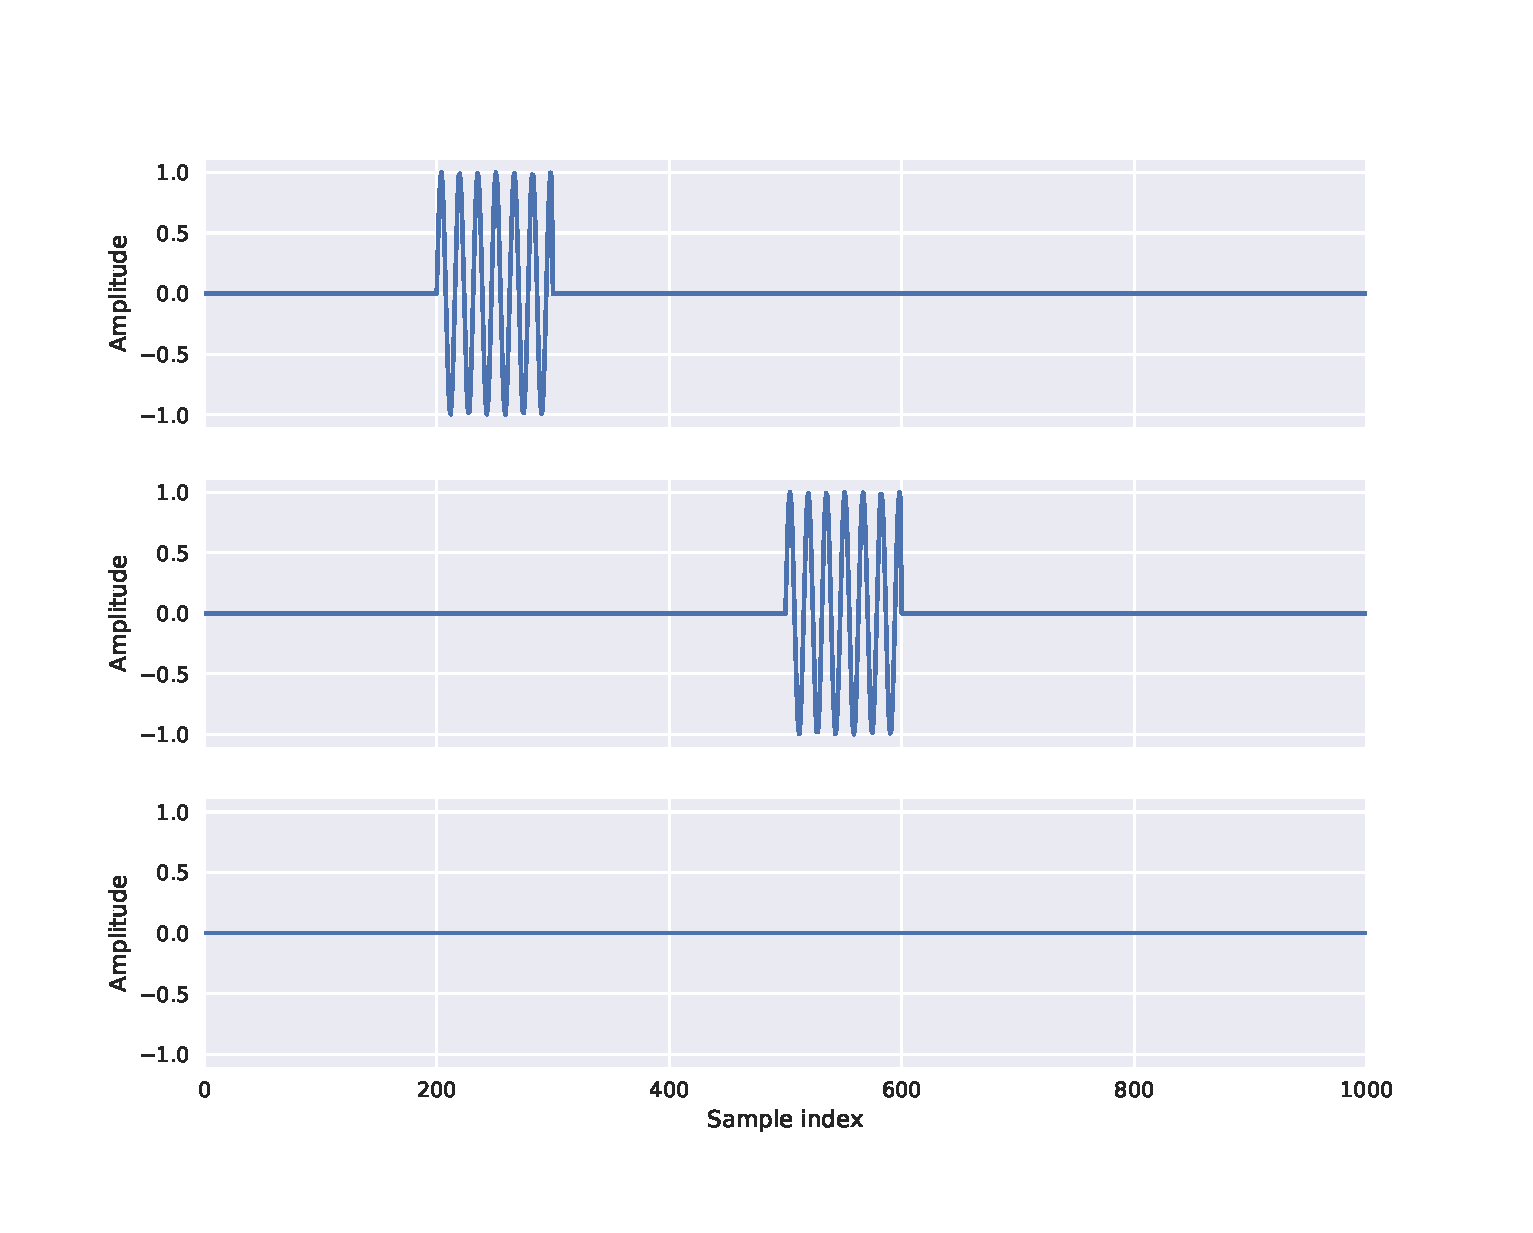
\includegraphics[scale=0.5]{figs_temp/mixing0}
	\caption{Analysis pulse $x_T(t-\tau)$ (top), received pulse $y(t)$ (mid) and multiplication output $x_T(t-\tau)y(t)$ (bot). As the signals do not overlap the multiplication yields only zero values.}
	\label{fig:mix0}
\end{figure}

\begin{figure}[t]
	\centering
	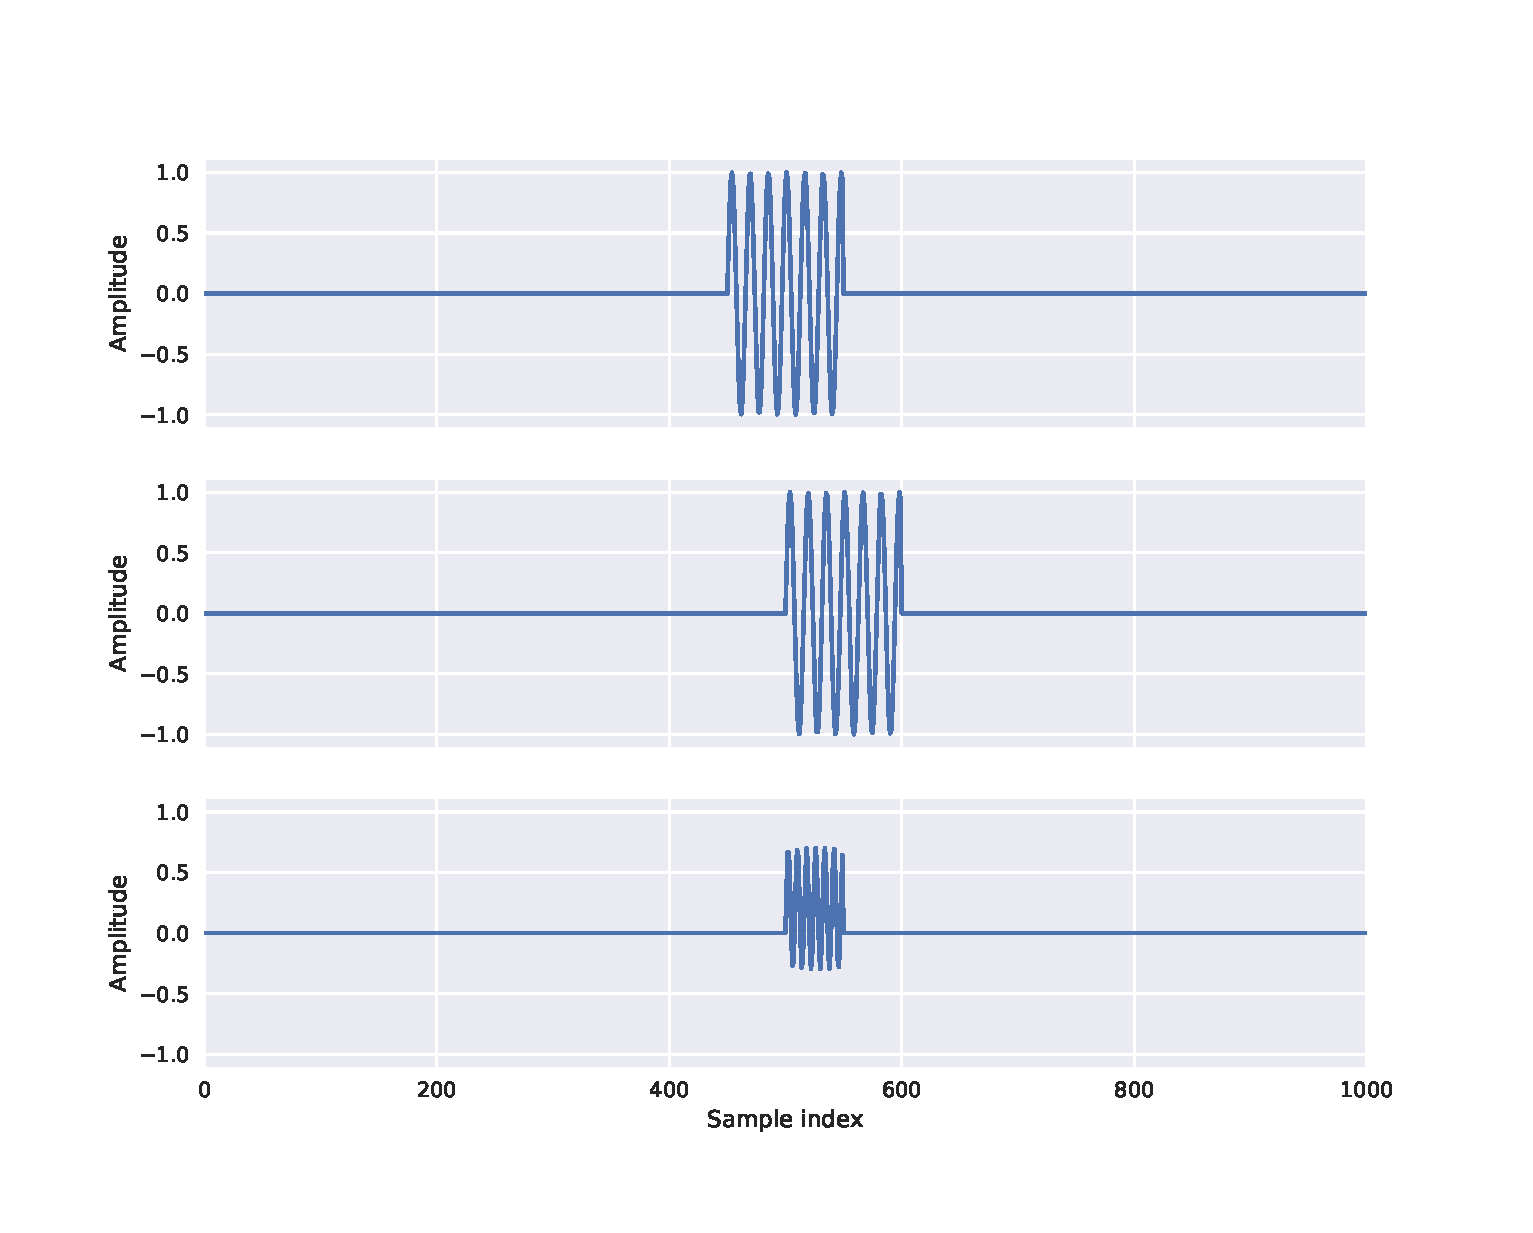
\includegraphics[scale=0.5]{figs_temp/mixing1}
	\caption{Analysis pulse $x_T(t-\tau)$ (top), received pulse $y(t)$ (mid) and multiplication output $x_T(t-\tau)y(t)$ (bot). The overlapping signals produce non-zero values after multiplication.}
	\label{fig:mix1}
\end{figure}

\begin{figure}[t]
	\centering
	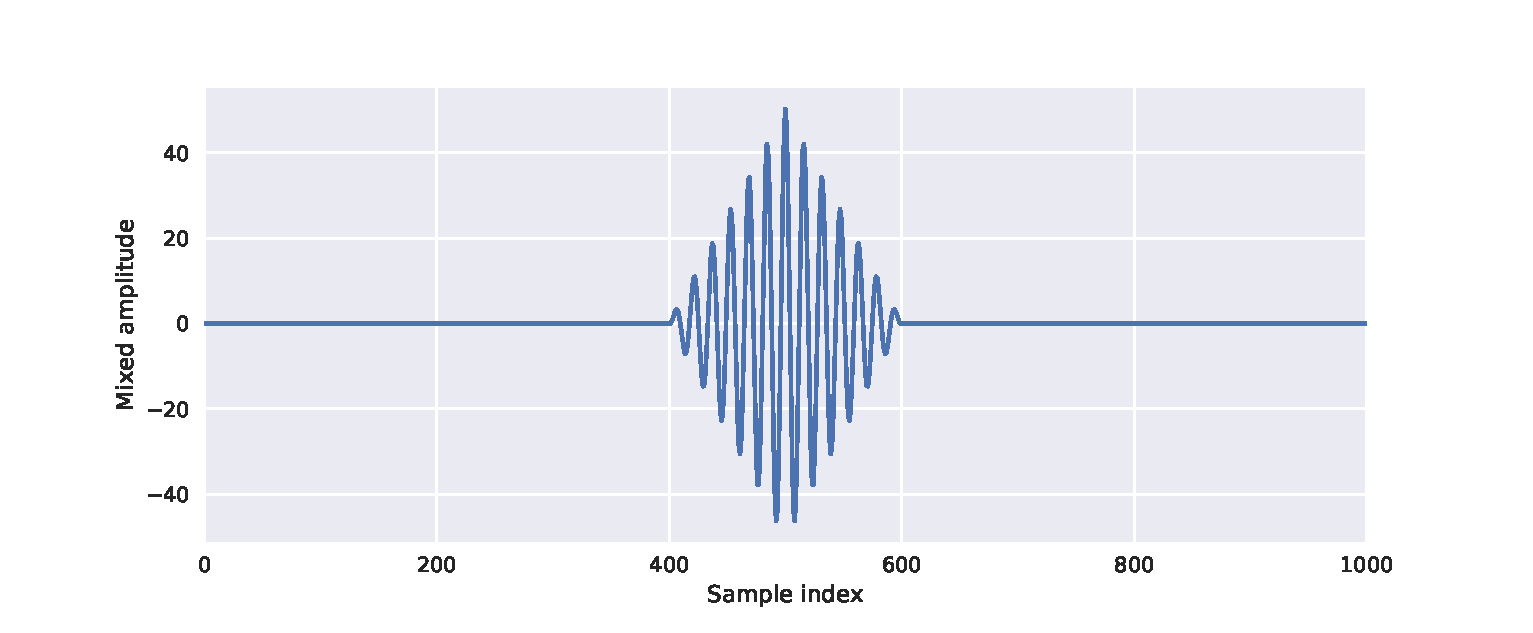
\includegraphics[scale=0.5]{figs_temp/mixing2}
	\caption{The matched filtering output $m(\tau)$ is produced by summing the overlap of the analysis and received pulse for all lags $\tau$.}
	\label{fig:mix2}
\end{figure}
\begin{equation}
	A(t) = \begin{cases}
		1 & \text{if $0\leq t < L$} \\
		0 & \text{otherwise},
	\end{cases}
\end{equation}

$m(\tau)$ will be on the form 
\begin{equation}\label{eq:n0}
	m(\tau) = 
	\begin{cases}
		0 & \text{if $|\tau-2d/c|\geq L$} \\
		\text{\eqref{eq:n1}} & \text{if $|\tau-2d/c|<L$ and $\tau \leq 2d/c$} \\
		\text{\eqref{eq:n2}} & \text{if $|\tau-2d/c|<L$ and $\tau > 2d/c$}
	\end{cases}
\end{equation}
\begin{equation}\label{eq:n1}
	\frac{C}{2}\Big((\tau + L - B)\cos(2\pi f_c(\tau - B)) 
	- \frac{1}{2\pi f_c}\sin(2\pi f_c(\tau - B))\Big)
\end{equation}
\begin{equation}\label{eq:n2}
	\frac{C}{2}\Big((B + L - \tau)\cos(2\pi f_c(\tau - B)) 
	+ \frac{1}{2\pi f_c}\sin(2\pi f_c(\tau - B))\Big).
\end{equation}

The full derivation of \eqref{eq:n0}, \eqref{eq:n1} and \eqref{eq:n2} can be found as an appendix. This procedure is illustrated in figures \ref{fig:mix0} and \ref{fig:mix1}. The analysis pulse is shown in the top plot, the received pulse in the center and the result of the elementwise multiplication at the bottom. These two figures differ in that the internal delay $\tau$ of the analysis pulse is different, so that no overlap occurs in the first figure while significant overlap happens in the second.

In figure \ref{fig:mix2} a numerical computation of $m(\tau)$ has been performed, shown in part in figures \ref{fig:mix0} and \ref{fig:mix1}. Note that this result was obtained for a noise-free mixing of a signal from a single theoretical point scattering target. It is thus clear that with complicated continuous structures, target scenes produce complex outputs at the receiver.

\section{IQ Demodulation}
\label{sec:iq}

Even though single-antenna receivers have no angular resolution, it was shown above that the returning signal carries useful information. By measuring the temporal shift from transmission to reception we can calculate the distance to a scatterer, and by examining the phase shift between pulses we may find the \gls{bf} and thus the radial velocity of the scatterer. Finally, the scatterers dielectric properties are brought forward through the \gls{rcs}, showing up as a scaling factor after matched filtering. 

Although the raw data signal produced by matched filtering holds the information we are interested in, it has commonly low \gls{snr} \citep{richards_2014} and holds the carrier frequency as can be seen in equations \eqref{eq:n0} to \eqref{eq:n2} and figure \ref{fig:mix2}. To this end, some transformation of the raw data signal is usually performed. In this work we are particularly interested in resolving small Doppler shifts, and thus we wish to closely monitor phase shifts from one measurement to the next. One effective data representation of raw data that facilitates accurate phase tracking involves splitting the signal into its \emph{In-phase} and \emph{Quadrature} (\gls{iq}) components \citep{lien_gillian_karagozler_amihood_schwesig_olson_raja_poupyrev_2016}. 

The In-phase channel mixes the raw signal with an oscillator at the carrier frequency $f_c$, and the Quadrature channel with the same frequency but with a $90^\circ$ phase shift from the I channel. After low-pass filtering, the \gls{iq} components are interpreted as a complex number $I(t) + jQ(t)$. \gls{iq} demodulation shifts the information bearing part of the mixed signal to baseband, meaning that an echo waveform on form $A(t)\sin(2\pi f_c t + \phi(t))$ after demodulation has form $A(t)e^{j\phi(t)}$, effectively eliminating the carrier frequency. Thus, after matched filtering and \gls{iq} demodulation we obtain a set of complex range measurements that we will denote as a \emph{radar sweep}. The details of the \gls{iq} demodulation scheme can be found in the appendix. 

%In figure \ref{fig:single_sweep_iq} the amplitude of a radar sweep is shown for data captured using the same measurement setup as in figure \ref{fig:single_sweep_raw}. Although the amplitude may be useful, the real power of splitting the signal into its I and Q constituents come from its phase tracking capabilities, as the phase is vastly more sensitive to small changes in range than the amplitude \citep{lien_gillian_karagozler_amihood_schwesig_olson_raja_poupyrev_2016}.

% Is this good enough?
% TODO: Incorporate more of what is written below. Intermediary frequency? Discuss with Peter. 


%A common type of data when working with radar signal processing is in-phase and quadrature-phase data (IQ-data). IQ-data is represented as complex numbers, and a radar sweep consists of several such complex numbers - one for each investigated range. The process of obtaining IQ-data is often referred to as IQ- or quadrature demodulation, and is described in appendix .... The usefulness of this type of data lies in that it contains explicit information about the amplitude, $A(t)$, and phase, $\theta(t)$, in equation \eqref{eq:raw_sweep} \citep{richards_2014}. To obtain the amplitude for a sweep, $s$, one simply computes the absolute value for each complex number in $s$. The amplitude plot is a good way to visualize at what ranges objects are present. Figure \ref{fig:single_sweep_iq} illustrates such a graph where the same measurement setup as in figure \ref{fig:single_sweep_raw} has been used. Similarly, a phase curve can be obtained by computing the phase in each point.

%In many applications, the phase information in IQ-data is used when small changes in the radar signal need to be detected, (Mention a case such as recording over grass...) as the phase is more sensitive to changes than the amplitude \citep{lien_gillian_karagozler_amihood_schwesig_olson_raja_poupyrev_2016}. If an object is detected at distance $r(t_1)$ from the radar at time $t_1$, and shortly thereafter, the object is moved to distance $r(t_2)$, the corresponding difference in phase will be
%\begin{equation}
%	\label{eq:phase_diff}
%	\Delta\phi(t_1, t_2)=\frac{4\pi}{\lambda}(r(t_2)-r(t_1)) \quad\quad \textrm{mod 2$\pi$}
%\end{equation}
%By having a sampling frequency which is too low, the range difference in $\eqenref{eq:phase_diff}$ could potentially become very big, and the phase difference would fluctuate over time and be incomprehensible.

%In the case of material classification, a high sampling frequency is highly beneficial. When moving across surfaces characterized by tiny details, a high sampling frequency is essential in capturing the shapes of these.
\iffalse
\begin{figure}[t]
	\centering
	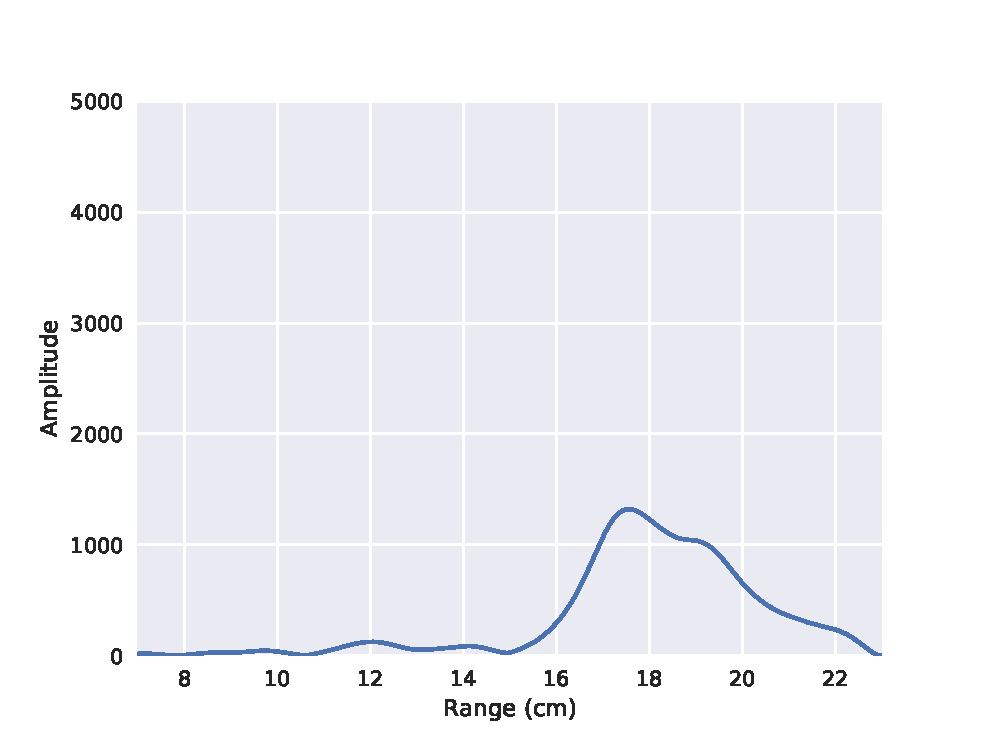
\includegraphics[scale=0.7]{figs_temp/single_sweep_iq}
	\caption{Absolute values of IQ data for .}
	\label{fig:single_sweep_iq}
\end{figure}
\fi
%For a thorough description of how IQ-data is derived, see appendix ...











%
%

